\documentclass[compress]{beamer}
\usepackage{ifthen,verbatim}

\newcommand{\isnote}{}
\xdefinecolor{lightyellow}{rgb}{1.,1.,0.25}
\xdefinecolor{darkblue}{rgb}{0.1,0.1,0.7}
\xdefinecolor{darkgreen}{rgb}{0.,0.6,0.}

%% Uncomment this to get annotations
%% \def\notes{\addtocounter{page}{-1}
%%            \renewcommand{\isnote}{*}
%% 	   \beamertemplateshadingbackground{lightyellow}{white}
%%            \begin{frame}
%%            \frametitle{Notes for the previous page (page \insertpagenumber)}
%%            \itemize}
%% \def\endnotes{\enditemize
%% 	      \end{frame}
%%               \beamertemplateshadingbackground{white}{white}
%%               \renewcommand{\isnote}{}}

%% Uncomment this to not get annotations
\def\notes{\comment}
\def\endnotes{\endcomment}

\setbeamertemplate{navigation symbols}{}
\setbeamertemplate{headline}{\mbox{ } \hfill
\begin{minipage}{5.5 cm}
\vspace{-0.75 cm} \small
\end{minipage} \hfill
\begin{minipage}{4.5 cm}
\vspace{-0.75 cm} \small
\begin{flushright}
\ifthenelse{\equal{\insertpagenumber}{1}}{}{Jim Pivarski \hspace{0.2 cm} \insertpagenumber\isnote/\pageref{numpages}}
\end{flushright}
\end{minipage}\mbox{\hspace{0.2 cm}}\includegraphics[height=1 cm]{../cmslogo} \hspace{0.1 cm} \includegraphics[height=1 cm]{../tamulogo} \hspace{0.01 cm} \vspace{-1.05 cm}}

\begin{document}
\begin{frame}
\vfill
\begin{center}
\textcolor{darkblue}{\Large Alignment of the CMS muon system \\ \vspace{0.15 cm}with beam halo and cosmic muon tracks}

\vfill
\begin{center}
\large
\textcolor{darkblue}{Jim Pivarski}

\scriptsize
\vspace{0.25 cm}
{\it Texas A\&M University}

\vspace{0.75 cm}
\small
\textcolor{darkblue}{on behalf of the CMS Collaboration}
\end{center}

\vfill
15 June, 2009

\end{center}
\end{frame}

%% \begin{notes}
%% \item This is the annotated version of my talk.
%% \item If you want the version that I am presenting, download the one
%% labeled ``slides'' on Indico (or just ignore these yellow pages).
%% \item The annotated version is provided for extra detail and a written
%% record of comments that I intend to make orally.
%% \item Yellow notes refer to the content on the {\it previous} page.
%% \item All other slides are identical for the two versions.
%% \end{notes}

\small

\begin{frame}
\frametitle{Outline}
\begin{itemize}\setlength{\itemsep}{0.65 cm}
\item Quick overview of the CMS muon system

\item Alignment of endcap chambers with LHC beam-halo tracks

\item Alignment of barrel chambers with CRAFT cosmic rays
\end{itemize}
%% \hspace{-0.83 cm} \textcolor{darkblue}{\Large Outline2}

\vfill
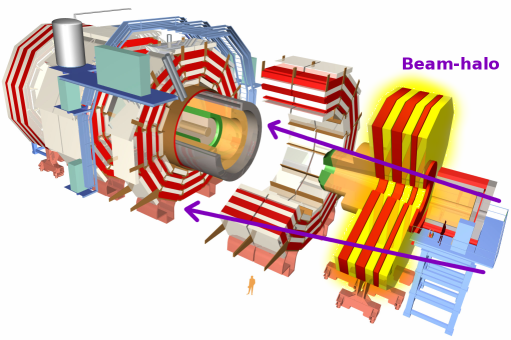
\includegraphics[width=0.47\linewidth]{CMS_exploded_endcap.png} \hfill 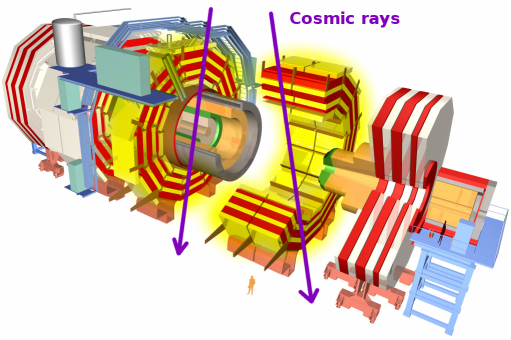
\includegraphics[width=0.47\linewidth]{CMS_exploded_barrel.png}
\end{frame}

\begin{frame}
\frametitle{CMS muon system}

\begin{itemize}
\item Tracking in modular chambers: 6 to 12 layers each
\item Global track formed from chambers' segments and \mbox{the silicon tracker\hspace{-1 cm}}
\end{itemize}

\begin{columns}
\column{0.7\linewidth}
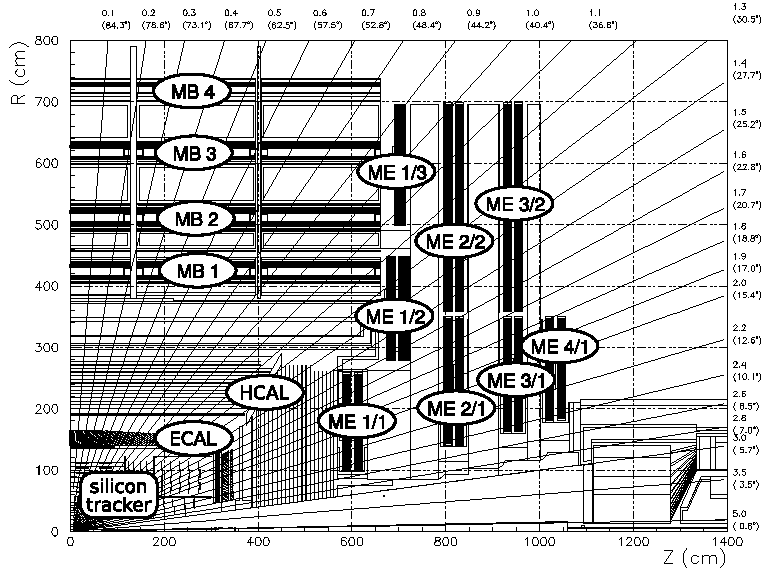
\includegraphics[width=\linewidth]{muon_system_labeled.pdf}

\column{0.3\linewidth}
\begin{itemize}
\item Barrel \mbox{(drift tube)} chambers grouped into 4~radial stations, 5~longitudinal wheels
\item Endcap \mbox{(cathode strip)} chambers grouped into 8~rings per endcap
\end{itemize}
\end{columns}

\begin{itemize}
\item This talk will be about aligning the individual chambers
\item Target for alignment is scale of $r\phi$ hit resolutions: $\mathcal{O}(\mbox{100--300~$\mu$m})$
\end{itemize}
\end{frame}

\begin{frame}
\frametitle{Beam-halo alignment method}

\vspace{-0.15 cm}
\begin{columns}
\column{0.75\linewidth}
\vspace{0.3 cm}
\begin{itemize}
\item Endcap muon chambers were designed with a small overlap region for alignment
\item Tracks passing through overlap region connect chambers without
  any intervening scattering material or long-distance propagation
\item High-precision relative \mbox{alignment of chamber pairs\hspace{-1 cm}}
\item Propagate pair corrections around \mbox{each ring with a simultaneous\hspace{-3 cm}} \\ solution of 18 (36) equations $\times$ 3 parameters \mbox{(1 translation, 2 angles)\hspace{-5 cm}}
\end{itemize}

\column{0.25\linewidth}
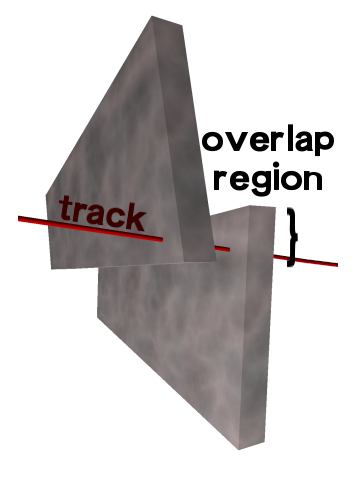
\includegraphics[width=0.8\linewidth]{overlaps.png}
\end{columns}

\vspace{0.1 cm}
\hfill 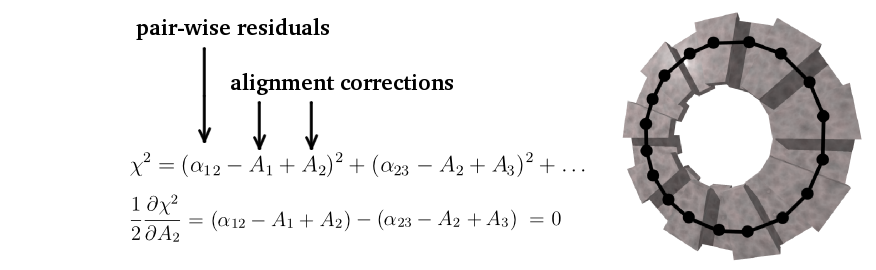
\includegraphics[width=0.8\linewidth]{matrix_description_onestation.png}

\mbox{\hspace{-0.45 cm}
\begin{minipage}{\linewidth}
\begin{itemize}
\item Followed by rigid-body alignment of internally-aligned ring with global tracks, to connect ring's coordinate system to silicon tracker
\end{itemize}
\end{minipage}}
\end{frame}

\begin{frame}
\frametitle{Test of method in Monte Carlo}

\begin{columns}
\column{0.65\linewidth}
\begin{itemize}
\item Procedure applied to Monte Carlo sample with statistics comparable to 2008 LHC single-beam run
\item Plot aligned-minus-true value for each of the 3 parameters, for every chamber (histogram entries are chambers)
\begin{itemize}
\item \mbox{RMS is the accuracy predicted by MC\hspace{-1 cm}}
\end{itemize}
\end{itemize}

\column{0.35\linewidth}
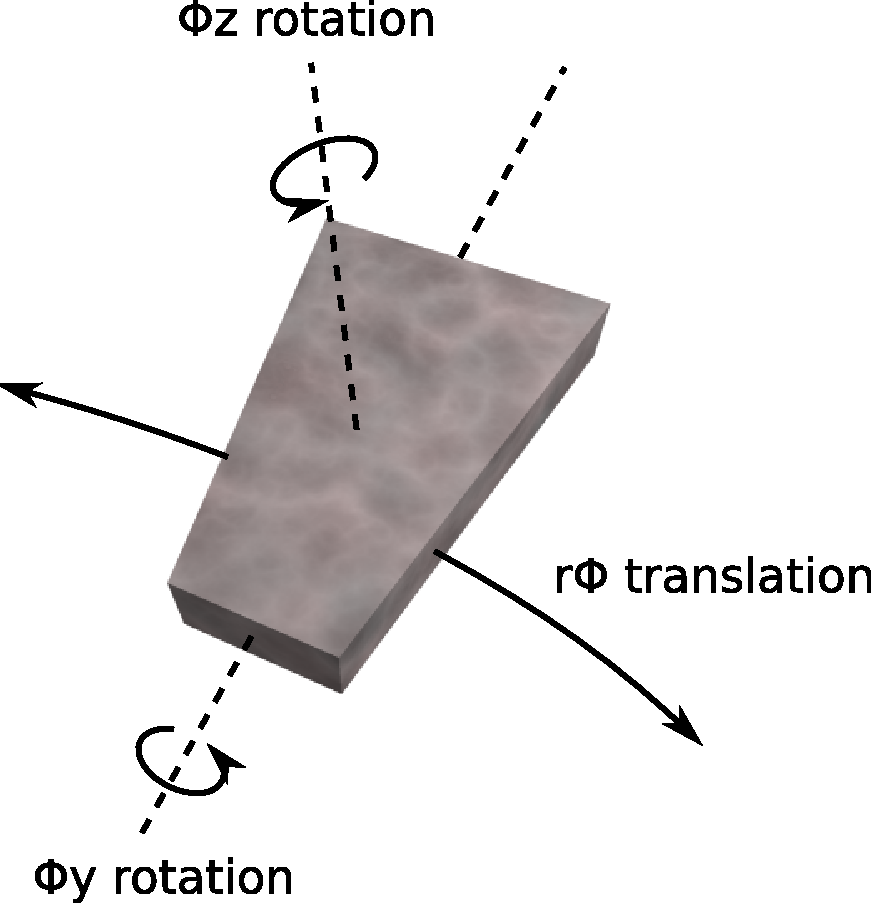
\includegraphics[width=\linewidth]{csc_coordinates.pdf}
\end{columns}

\vfill
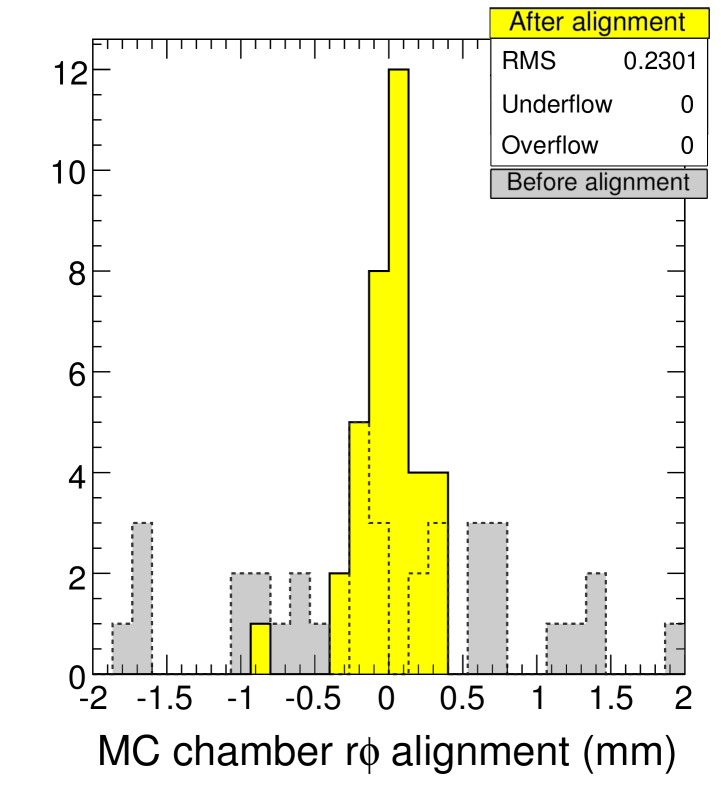
\includegraphics[width=0.33\linewidth]{mc_rphi.png}
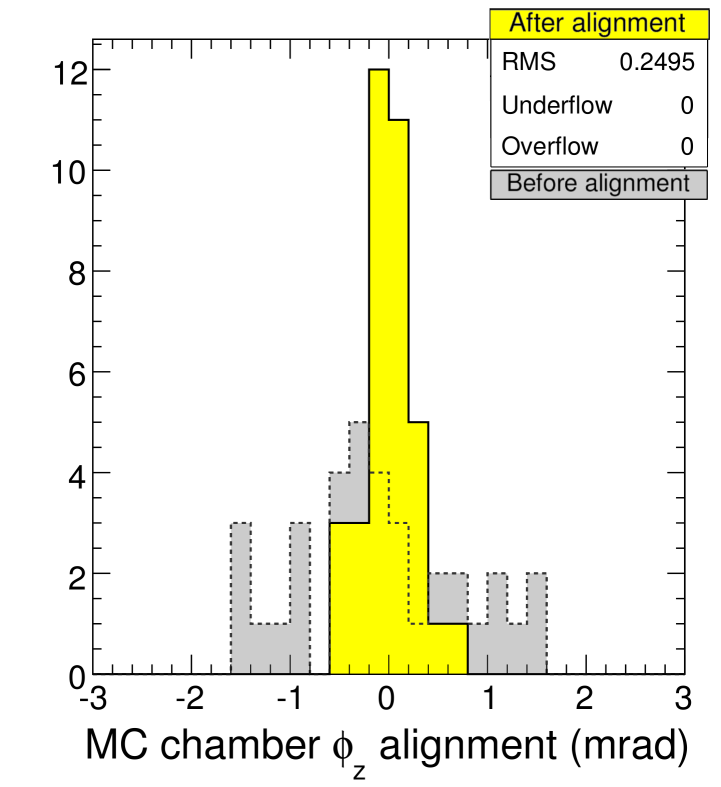
\includegraphics[width=0.33\linewidth]{mc_phiz.png}
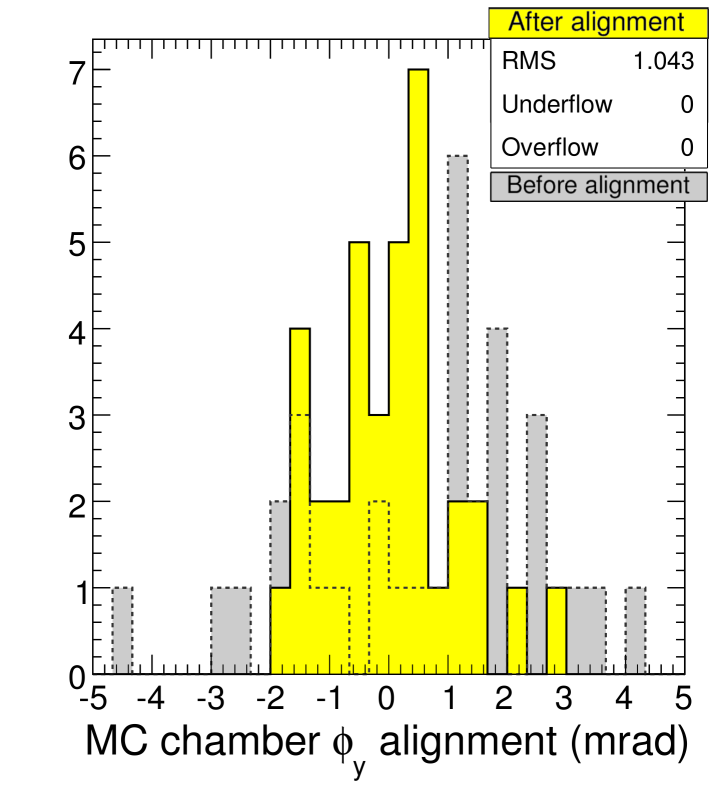
\includegraphics[width=0.33\linewidth]{mc_phiy.png}

\end{frame}

\begin{frame}
\frametitle{2008 LHC beam-halo data}

\begin{columns}
\column{0.35\linewidth}
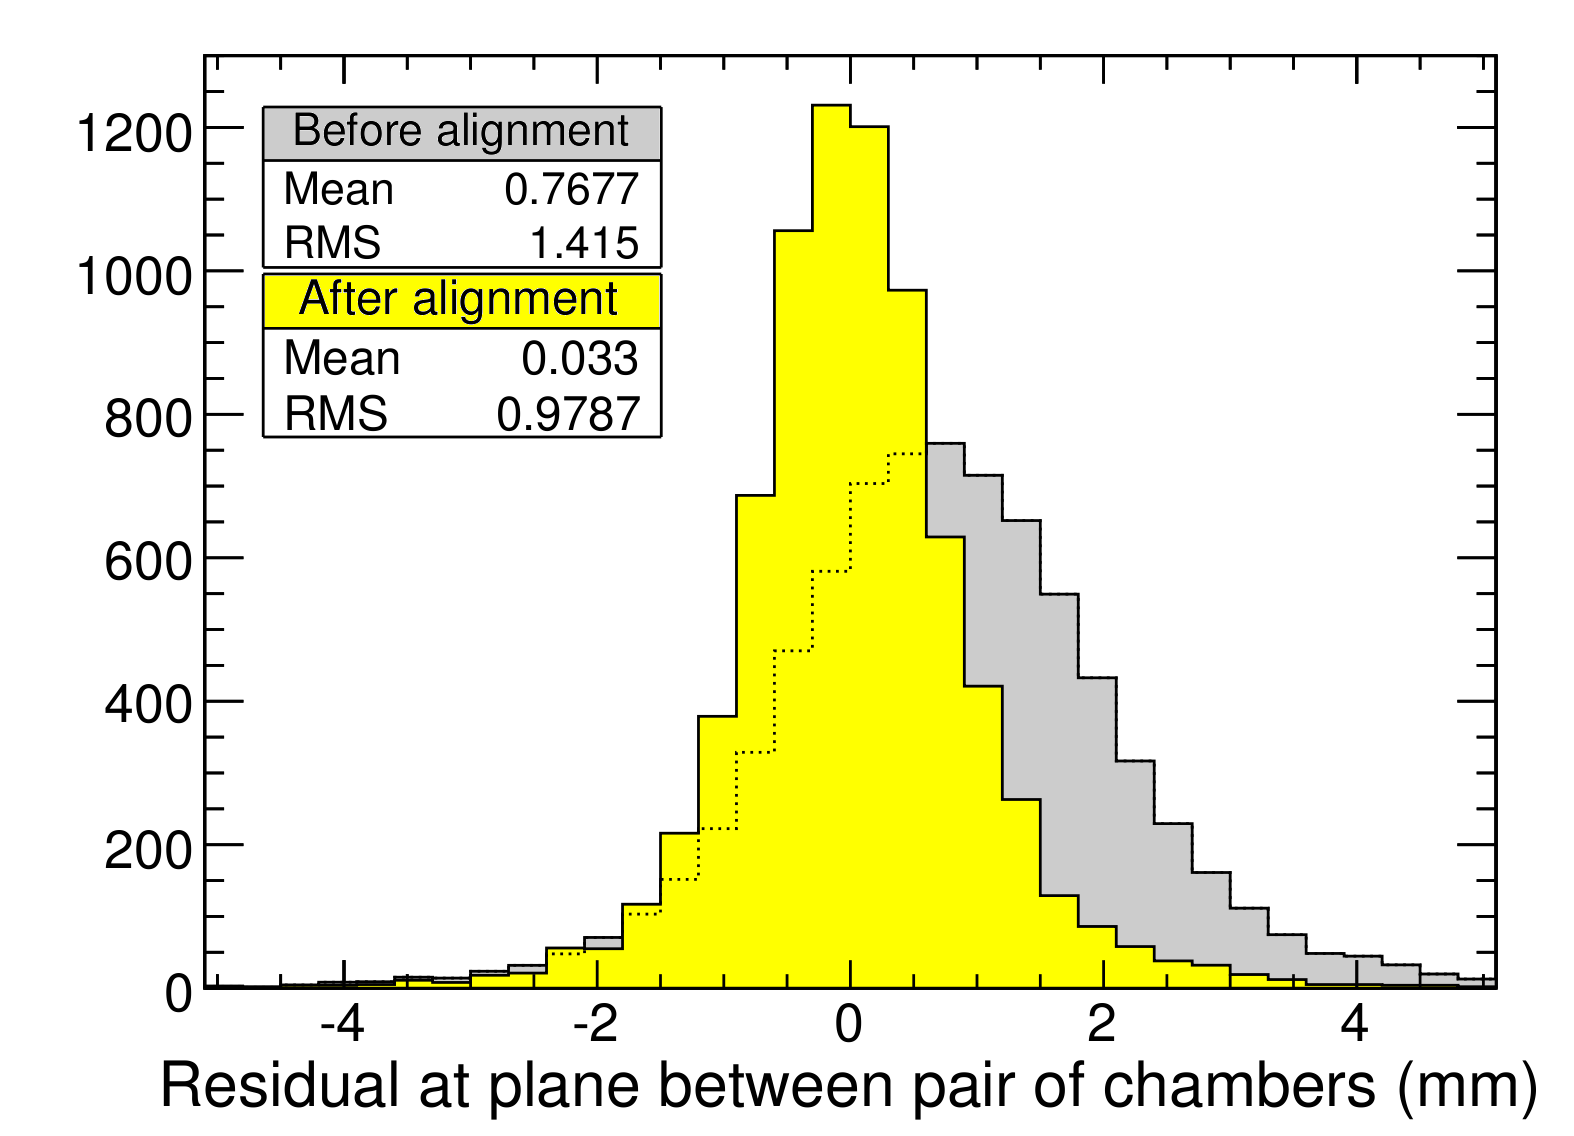
\includegraphics[width=\linewidth]{residuals_just_before_and_after.png}

\vspace{0.25 cm}
\column{0.6\linewidth}
\begin{itemize}
\item Procedure applied to September 2008 LHC beam-halo dataset
\item ME$-$2/1 and ME$-$3/1 only \\ (highest statistics from beam-2)
\item Narrows and centers residuals distribution (left)
\end{itemize}
\end{columns}

\vspace{0.1 cm}
\mbox{\hspace{-0.45 cm}
\begin{minipage}{\linewidth}
\begin{itemize}
\item Verified by independent photogrammetry: alignment from a literal photograph of \mbox{the detector\hspace{-1 cm}}
\end{itemize}
\end{minipage}}

\vspace{0.2 cm}
\begin{columns}
\column{0.25\linewidth}
\vspace{-1 cm}
\begin{itemize}
\item Both saw corrections relative to the design description, with high correlation
\end{itemize}

\column{0.75\linewidth}
\hfill 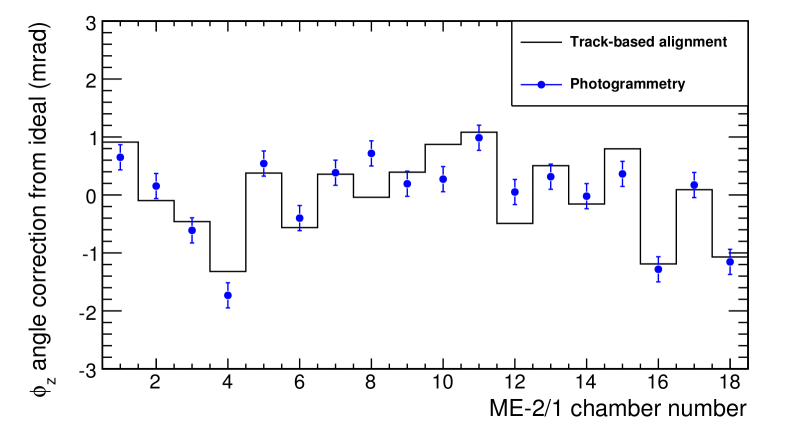
\includegraphics[width=0.95\linewidth]{data_correlations.png}
\end{columns}
\end{frame}

\begin{frame}
\frametitle{2008 LHC beam-halo data}

\vspace{0.2 cm}
\mbox{\hspace{-0.5 cm}\begin{minipage}{\linewidth}
\begin{itemize}
\item Chamber-by-chamber comparisons with photogrammetry (PG):
\begin{itemize}\setlength{\itemsep}{0.1 cm}
\item agreement with \textcolor{darkblue}{270~$\mu$m} position and \textcolor{darkblue}{0.35~mrad} \mbox{angular accuracy\hspace{-1 cm}}
\item close to the 166~$\mu$m intrinsic hit uncertainty \mbox{(for these chambers)\hspace{-1 cm}}
\item 33,000 events from a \textcolor{darkblue}{9-minute} long run \mbox{($\frac{3}{4}$ of 2008 beam data)\hspace{-2 cm}}
\end{itemize}
\end{itemize}
\end{minipage}}

\vspace{0.4 cm}
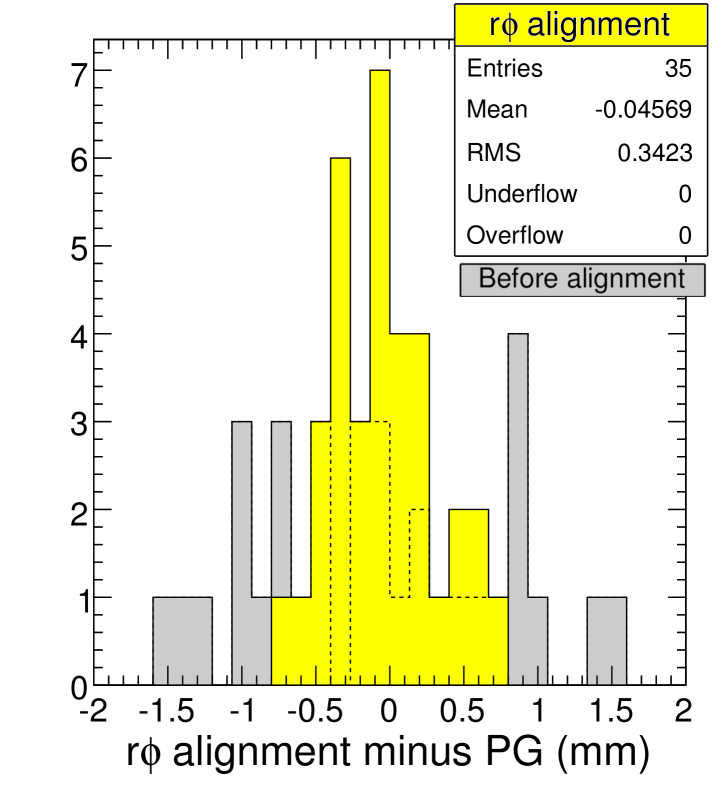
\includegraphics[width=0.5\linewidth]{data_rphi.png}
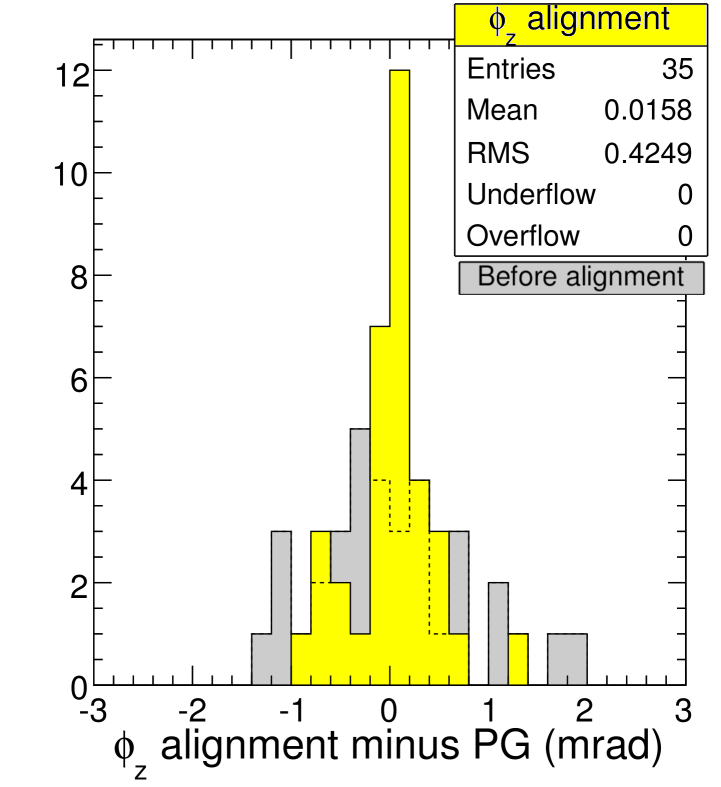
\includegraphics[width=0.5\linewidth]{data_phiz.png}
\end{frame}

\begin{frame}
\frametitle{Global muon alignment}

\vspace{0.5 cm}
\begin{columns}
\column{0.6\linewidth}
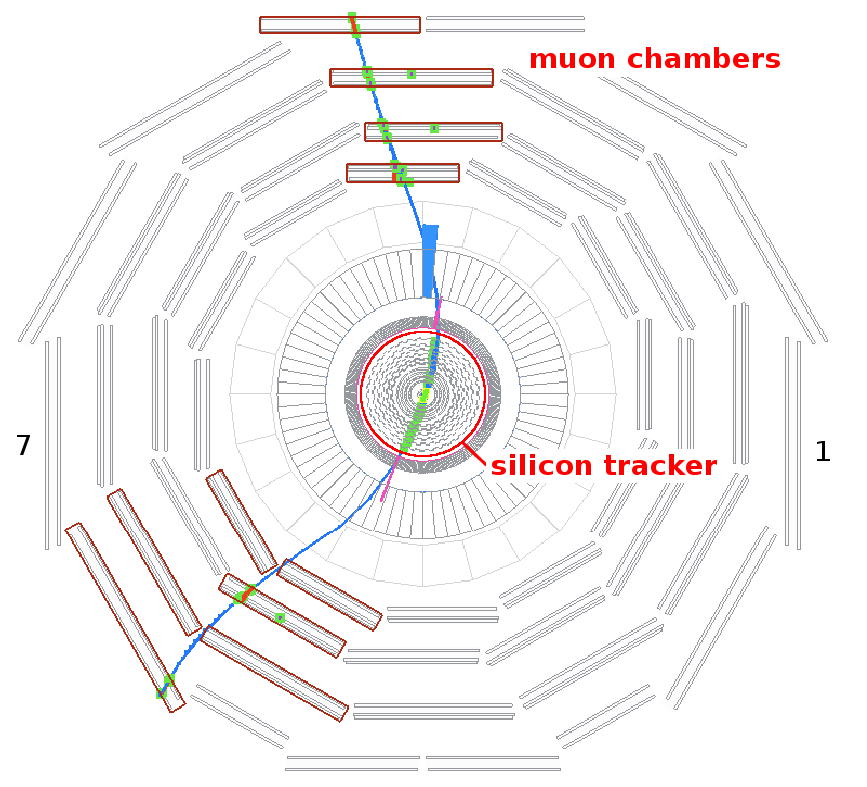
\includegraphics[width=\linewidth]{event_display.png}

\column{0.4\linewidth}
\hspace{-0.4 cm} \textcolor{darkblue}{\large Goal}
\begin{itemize}
\item Obtain consistent, CMS-wide coordinate system in one step
\end{itemize}

\vspace{0.2 cm}
\hspace{-0.4 cm} \textcolor{darkblue}{\large Method}

\begin{itemize}
\item Select tracks that pass through muon chambers and tracker
\item Fit track using tracker information only
\item Align chamber to optimize residuals
\end{itemize}
\end{columns}

\vspace{0.25 cm}
\begin{itemize}
\item Can be applied to all chambers using collisions muons, and most barrel chambers with CRAFT cosmic rays (central wheels \mbox{$-$1, 0, $+$1,\hspace{-0.5 cm}} \\ all sectors except the horizontal ones: 1 and 7)
\end{itemize}
\end{frame}

\begin{frame}
\frametitle{Chamber residuals}

\begin{columns}
\column{0.6\linewidth}
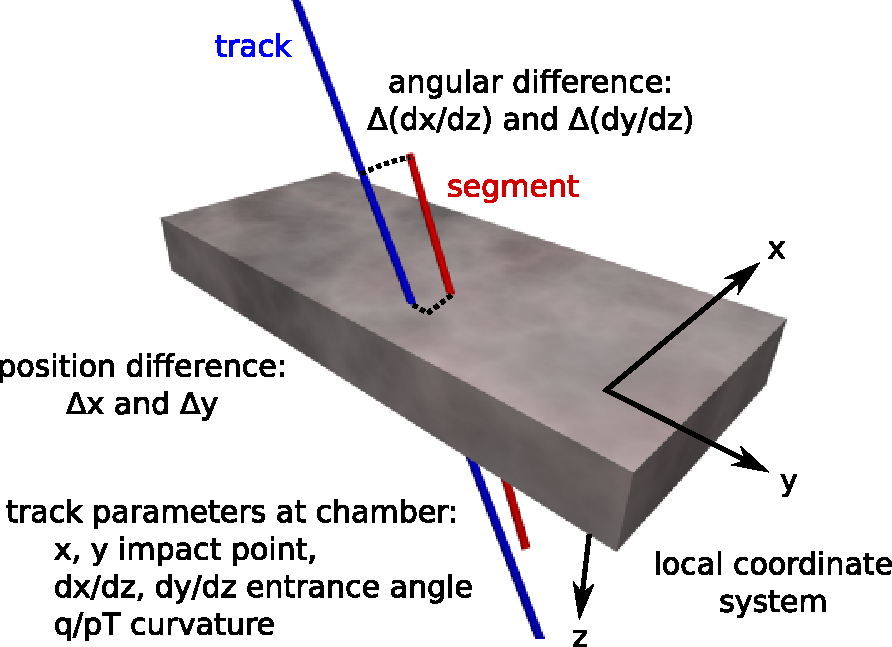
\includegraphics[width=\linewidth]{dt_coordinates.pdf}

\column{0.4\linewidth}
\begin{itemize}
\item \mbox{Chamber measures 2-D\hspace{-1 cm}} \\ position and direction: 4-component residuals
\item Access to 6 rigid-body alignment parameters \mbox{(3~translation, 3~rotation)\hspace{-0.5 cm}} through a $6\times 4$ derivatives matrix
\end{itemize}
\end{columns}

\vspace{0.75 cm}
\hspace{-0.83 cm} \textcolor{darkblue}{\Large Alignment fit}

\vfill
\begin{itemize}
\item Single fit function for each chamber, including all geometric and propagation effects
\item Project 8-dimensional, 16-parameter fit onto all coordinates for validation
\end{itemize}
\end{frame}

\begin{frame}
\frametitle{Sample fit results: \only<1>{MC}\only<2>{CRAFT data}}

\vspace{0.25 cm}
\begin{columns}
\column{0.5\linewidth}

\mbox{ } \hfill \textcolor{darkblue}{Before alignment} \hfill \mbox{ }

\only<1>{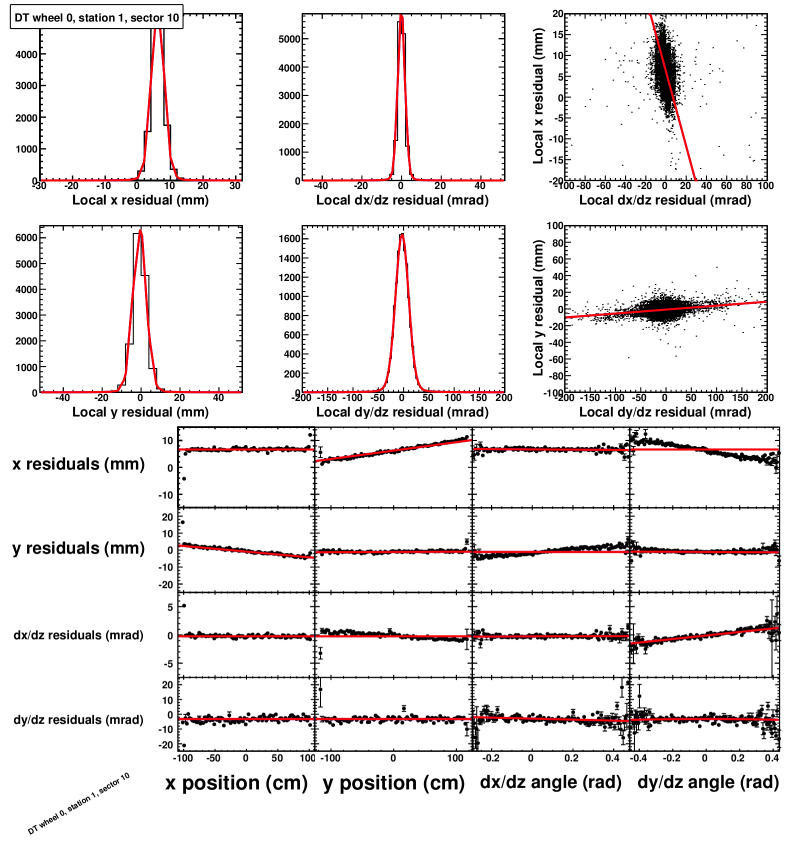
\includegraphics[width=\linewidth]{exampleMC_wh0st1sec10_before.png}}\only<2>{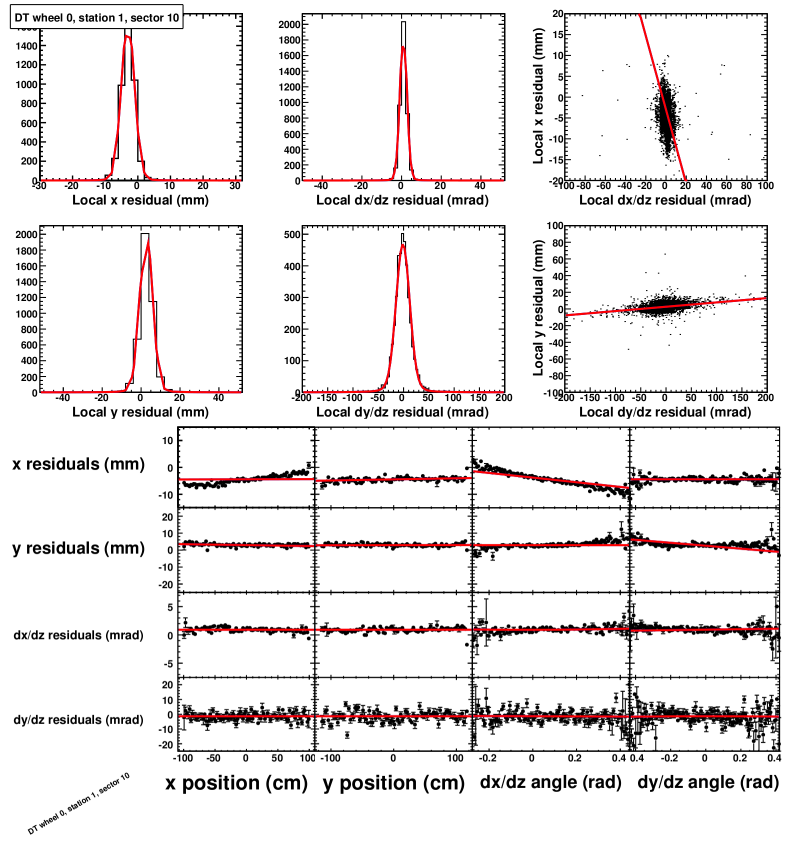
\includegraphics[width=\linewidth]{exampleData_wh0st1sec10_before.png}}

\column{0.5\linewidth}

\mbox{ } \hfill \textcolor{darkblue}{After alignment} \hfill \mbox{ }

\only<1>{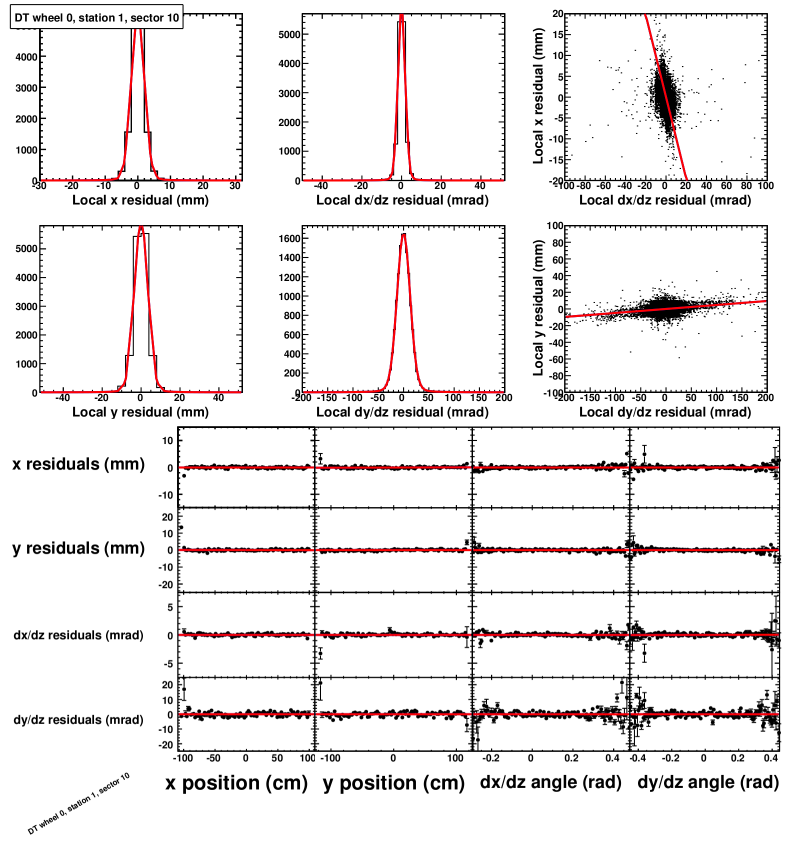
\includegraphics[width=\linewidth]{exampleMC_wh0st1sec10_after.png}}\only<2>{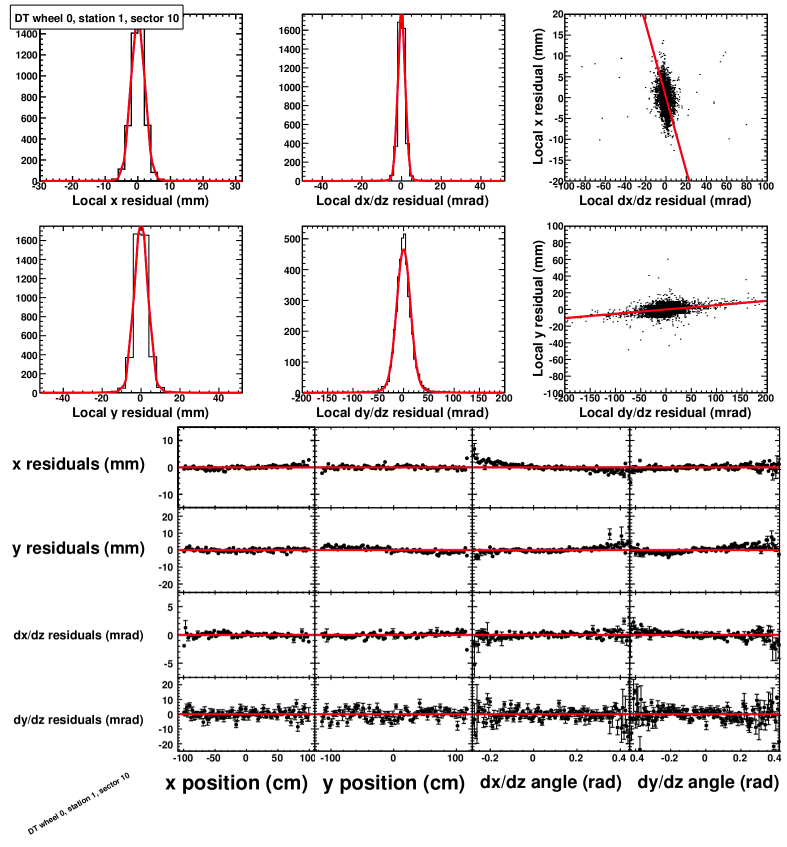
\includegraphics[width=\linewidth]{exampleData_wh0st1sec10_after.png}}

\end{columns}

\begin{itemize}
\item Projection of \textcolor{red}{fits (all parameters = 0 other than the one shown)} overlaid on {\it \only<1>{simulated}\only<2>{real}} data (profile plots) for \only<1>{one}\only<2>{the same} chamber
\item \only<1>{Method works well in Monte Carlo}\only<2>{Largely the same behavior in data; studying small discrepancies}
\end{itemize}
\end{frame}

\begin{frame}
\frametitle{MC cosmic ray results}

\begin{itemize}
\item Plot aligned-minus-true value of each of the 6 parameters for every chamber (histogram entries are chambers)
\begin{itemize}
\item predicted resolution for local $x$ (global $r\phi$) is 200~$\mu$m
\item CRAFT and MC are both systematics dominated
\end{itemize}
\item \textcolor{red}{MC tracker geometry is ideal:} this demonstrates
  the reach of the muon alignment method, given a well-aligned tracker
\end{itemize}

\begin{center}
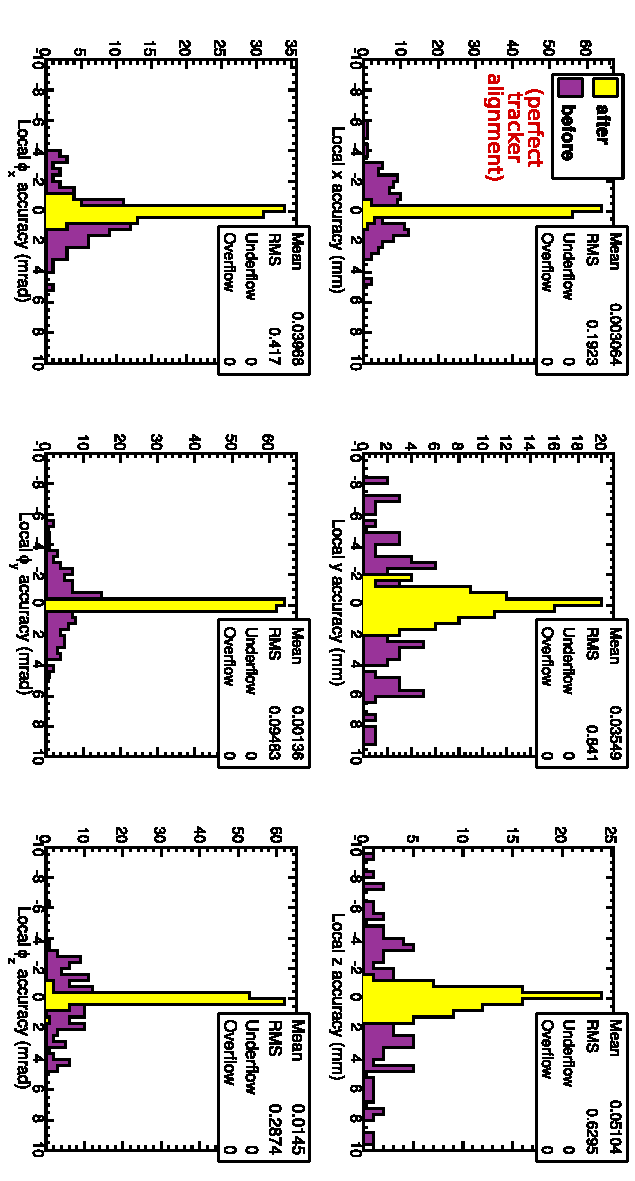
\includegraphics[height=0.9\linewidth, angle=90]{hip_MC_simple2.pdf}
\end{center}
\end{frame}

\begin{frame}
\frametitle{Data-driven $p_T$ resolution}

\begin{itemize}
\item Split $p_T \gtrsim 200$~GeV cosmic rays into upper and lower halves, refit each half independently and compare the results
\item Two track-fits for each cosmic ray: any mismatch is instrumental
\end{itemize}

\vspace{-0.5 cm}
\begin{columns}
\column{0.5\linewidth}
\begin{center}
\textcolor{darkblue}{Before muon alignment}

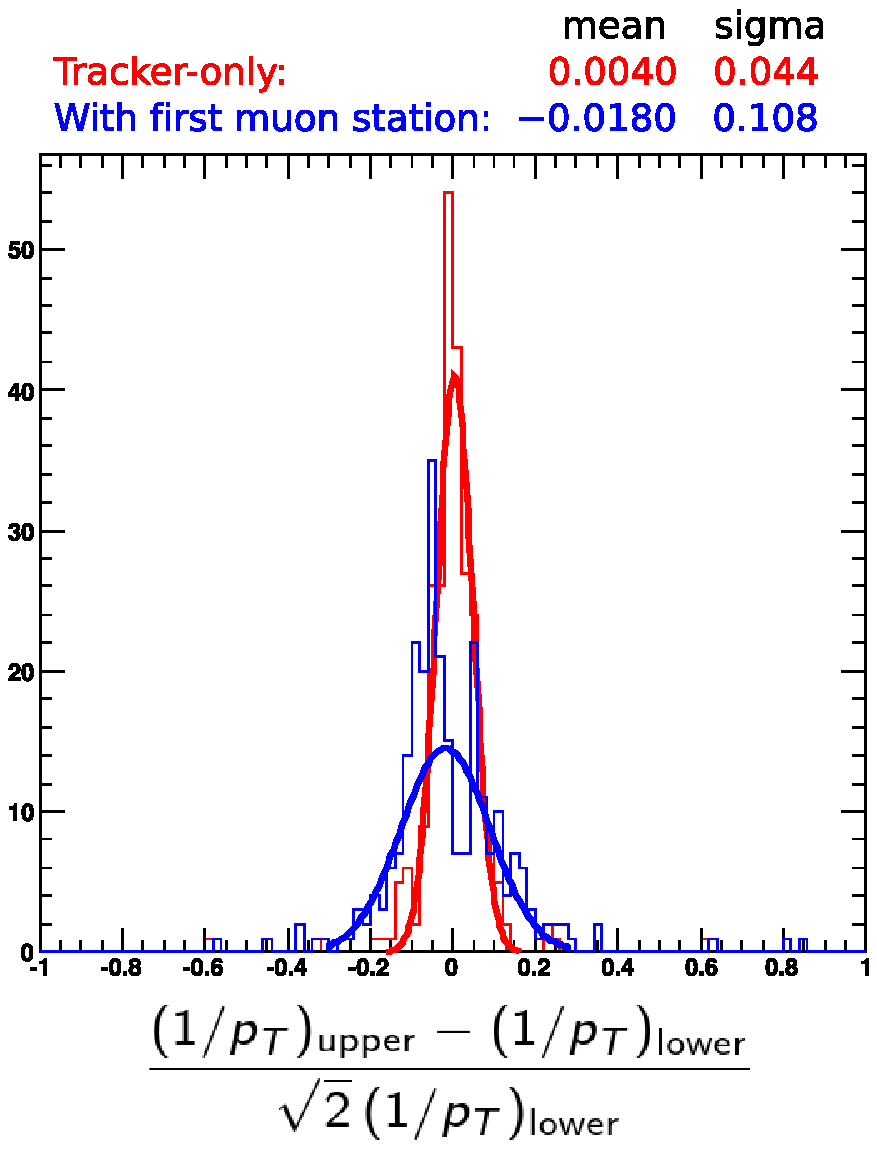
\includegraphics[width=0.9\linewidth]{without_alignment.pdf}
\end{center}
\column{0.5\linewidth}
\begin{center}
\textcolor{darkblue}{After muon alignment}

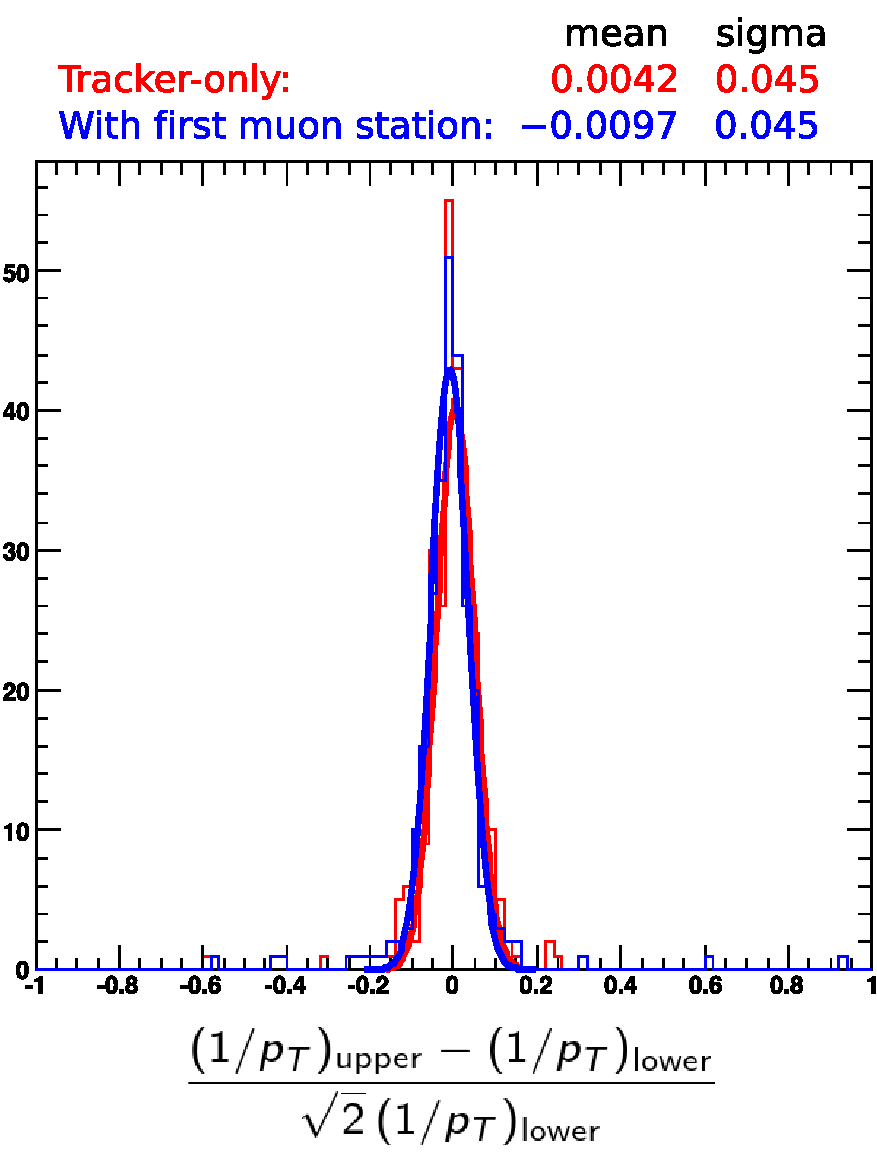
\includegraphics[width=0.9\linewidth]{with_alignment.pdf}
\end{center}
\end{columns}
\end{frame}

\begin{frame}
\frametitle{Comparison with expectations}

\begin{itemize}
\item MC resolution vs.~$p_T$ with different alignment scenarios
\item Track reconstruction method optimized by $p_T$

\mbox{\scriptsize (at high $p_T$, use only first muon station to avoid hit confusion from muon showering)\hspace{-1 cm}}
\end{itemize}

\vspace{-0.15 cm}
\begin{center}
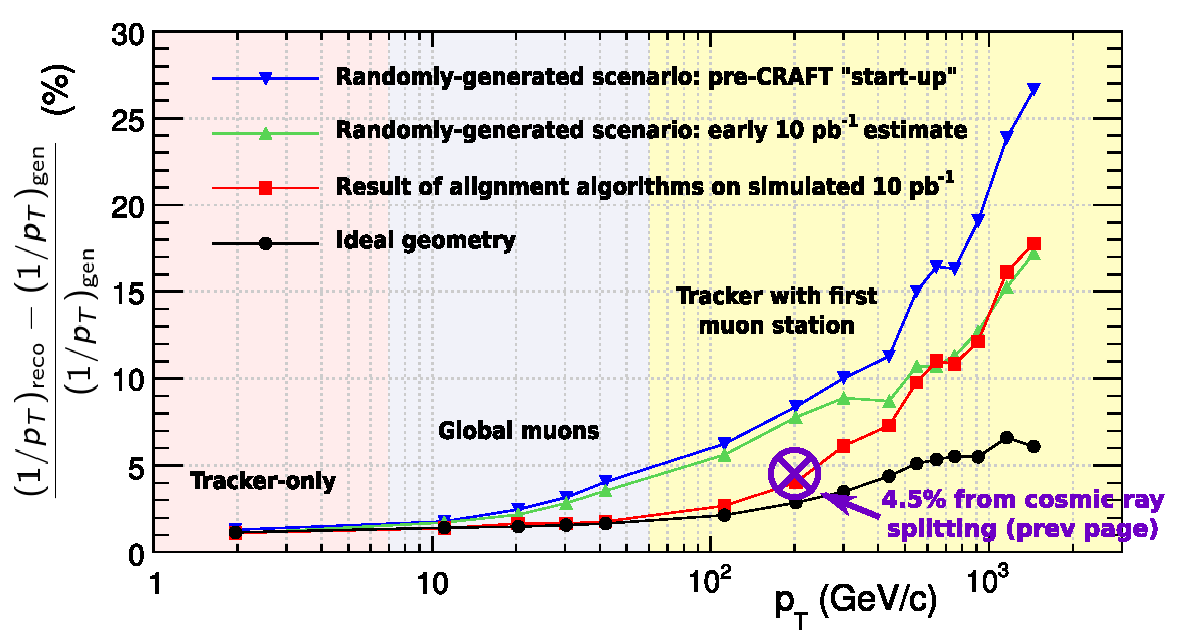
\includegraphics[width=0.9\linewidth]{curvature_resolution_cosmicpoint.pdf}
\end{center}

\vspace{-0.35 cm}
\begin{itemize}
\item \textcolor{red}{MC simulations} yield much better results than \mbox{\textcolor{darkgreen}{early estimates}\hspace{-1 cm}}
\item Cosmic ray splitting is close to MC simulations at 200~GeV
\end{itemize}
\end{frame}

%% \section*{First section}
%% \begin{frame}
%% \begin{center}
%% \Huge \textcolor{blue}{First section}
%% \end{center}
%% \end{frame}

\begin{frame}
\frametitle{Conclusions}

\begin{itemize}\setlength{\itemsep}{0.5 cm}
\item Track-based alignment methods were successfully applied to 2008 LHC beam-halo and CRAFT cosmic ray muons
\item High resolution predicted by Monte Carlo, supported by data-driven measurements
\item Pre-collisions alignments offer significantly improved tracking for the 2009 start-up
\item They also demonstrate that tools and procedures are ready for alignment with collisions muons
\end{itemize}

\label{numpages}
\end{frame}

\end{document}
